% !TEX program = lualatex
% ═══════════════════════════════════════════════════════════════════════
%  Chapitre 1 — Les transformations du plan
%  Diaporama Beamer pour un exposé magistral (~4-5 heures)
%  Jérôme Soucy — MAT-2901
%
%  Compilation : lualatex main.tex   (deux passages, pour le sommaire)
%
%  Ce diaporama reprend les définitions, propositions/théorèmes (énoncés
%  seulement), exemples, figures et tableaux du chapitre 1 des notes de
%  cours. Les démonstrations ne sont PAS reproduites : chaque résultat
%  qui, dans les notes, porte une démonstration est plutôt marqué
%  « DÉMONSTRATION AU TABLEAU », avec un rappel très court de l'idée, à
%  l'intention de la personne qui présente.
% ═══════════════════════════════════════════════════════════════════════
\documentclass[aspectratio=169, 11pt]{beamer}
% ═══════════════════════════════════════════════════════════════════════
%  preambule.tex — Réglages, couleurs et raccourcis communs du diaporama
%  du chapitre 1 (« Les transformations du plan »).
%  Ce fichier est autonome : il ne dépend d'aucun fichier du livre.
% ═══════════════════════════════════════════════════════════════════════

% ── Encodage, langue, polices (lualatex, comme le livre) ───────────────
\usepackage{fontspec}
\usepackage[french]{babel}

\setmainfont{TeX Gyre Termes}
\IfFontExistsTF{Fira Sans}
  {\setsansfont{Fira Sans}[Scale=MatchLowercase]}
  {\setsansfont{TeX Gyre Heros}[Scale=MatchLowercase]}
\usefonttheme{professionalfonts}
\renewcommand{\familydefault}{\sfdefault}

\usepackage{unicode-math}
\IfFontExistsTF{NewCMMath-Book.otf}
  {\setmathfont{NewCMMath-Book}}
  {\setmathfont{Latin Modern Math}}

\usepackage{amsmath}
\usepackage{mathtools}
\usepackage{booktabs}
\usepackage{array}
\usepackage{graphicx}
\usepackage{adjustbox}
\usepackage[skins,breakable]{tcolorbox}
\usepackage{tikz}
\usetikzlibrary{calc, arrows.meta, angles, quotes, patterns, positioning,
                decorations.markings, backgrounds, fit, shapes.geometric}

% ── Palette (identique à celle du livre, livrejs.cls) ──────────────────
\definecolor{sectioncolor}{RGB}{28, 63, 110}   % bleu foncé — titres
\definecolor{thmboxbg}{RGB}{228, 238, 252}     % bleu pâle — énoncés
\definecolor{coveraccent}{RGB}{196, 142, 58}   % or chaud — accent
\definecolor{secboxbg}{RGB}{253, 240, 219}     % ocre pâle — « Pour la classe »
\definecolor{steelblue4}{HTML}{36648B}         % figures : objet de départ
\definecolor{firebrick3}{HTML}{CD3333}         % figures : objet image
\definecolor{demobg}{RGB}{247, 247, 247}       % fond neutre — « au tableau »
\definecolor{bgpage}{RGB}{253, 253, 252}       % fond de diapositive, légèrement chaud

% ── Thème beamer : sobre, cohérent avec le livre ────────────────────────
\usecolortheme{default}
\setbeamercolor{palette primary}{bg=sectioncolor, fg=white}
\setbeamercolor{palette secondary}{bg=sectioncolor, fg=white}
\setbeamercolor{palette tertiary}{bg=sectioncolor, fg=white}
\setbeamercolor{title}{fg=sectioncolor}
\setbeamercolor{frametitle}{bg=sectioncolor, fg=white}
\setbeamercolor{structure}{fg=sectioncolor}
\setbeamercolor{section in toc}{fg=sectioncolor}
\setbeamercolor{subsection in toc}{fg=black}
\setbeamercolor{background canvas}{bg=bgpage}
\setbeamercolor{footline}{fg=gray, bg=bgpage}
\setbeamercolor{block title}{bg=sectioncolor, fg=white}
\setbeamercolor{block body}{bg=thmboxbg, fg=black}
\setbeamercolor{item}{fg=sectioncolor}
\setbeamercolor{itemize item}{fg=coveraccent}
\setbeamercolor{itemize subitem}{fg=sectioncolor}
\setbeamertemplate{itemize item}{\raise0.3ex\hbox{\small$\blacktriangleright$}}
\setbeamertemplate{itemize subitem}{\raise0.3ex\hbox{\footnotesize$\bullet$}}
\setbeamertemplate{navigation symbols}{}
\setbeamerfont{frametitle}{series=\bfseries}
\setbeamertemplate{frametitle}{%
  \vskip-1ex
  \begin{beamercolorbox}[wd=\paperwidth,ht=3.8ex,dp=1.3ex,leftskip=1em,rightskip=1em]{frametitle}
    \bfseries\strut\insertframetitle
  \end{beamercolorbox}
  \vskip3pt
}
\setbeamertemplate{footline}{%
  \leavevmode
  \hbox{\begin{beamercolorbox}[wd=\paperwidth,ht=2.4ex,dp=1ex,leftskip=1em,rightskip=1em]{footline}
    {\scriptsize\color{gray}Chapitre 1 --- Les transformations du plan
    \hfill \insertshorttitle{} \hfill \insertframenumber/\inserttotalframenumber}
  \end{beamercolorbox}}%
}
\setbeamertemplate{blocks}[rounded][shadow=false]
\setbeamertemplate{section in toc}{%
  \inserttocsectionnumber.~\inserttocsection\par\vskip0.15em}

% ── Page de section : diapositive de transition ────────────────────────
\AtBeginSection[]{%
  \begin{frame}[plain,c]
    \begin{center}
      {\color{coveraccent}\rule{0.25\textwidth}{1.2pt}}\\[10pt]
      {\usebeamerfont{frametitle}\usebeamercolor[fg]{title}%
       \Large\bfseries\color{sectioncolor}\insertsectionhead}\\[10pt]
      {\color{sectioncolor}\rule{0.45\textwidth}{0.5pt}}
    \end{center}
  \end{frame}
}
\AtBeginSubsection[]{%
  \begin{frame}[plain,c]
    \begin{center}
      {\large\color{gray}\insertsectionhead}\\[4pt]
      {\Large\bfseries\color{coveraccent}\insertsubsectionhead}
    \end{center}
  \end{frame}
}

% ── Raccourcis mathématiques repris du livre (autonomes) ────────────────
\newcommand{\Plan}{\Pi}
\newcommand{\Transf}{\mathcal{T}}
\newcommand{\Aff}{\mathcal{A}}
\newcommand{\Sim}{\mathcal{S}}
\newcommand{\Iso}{\mathcal{I}}
\newcommand{\mat}[4]{\begin{pmatrix}#1 & #2\\ #3 & #4\end{pmatrix}}
\newcommand{\col}[2]{\begin{pmatrix}#1\\ #2\end{pmatrix}}
\newcommand{\coliii}[3]{\begin{pmatrix}#1\\ #2\\ #3\end{pmatrix}}
\newcommand{\norme}[1]{\lVert #1 \rVert}
\newcommand{\Aire}{\operatorname{Aire}}
\newcommand{\dete}{\operatorname{det}}
\renewcommand{\vec}[1]{\mathbf{#1}}
\DeclareMathOperator{\R}{\mathbb{R}}
\DeclareMathOperator{\Rs}{\mathbb{R}^{\star}}
\newcommand{\intff}[2]{\mathopen{[}{#1},{#2}\mathclose{]}}
\newcommand{\intoo}[2]{\mathopen{]}{#1},{#2}\mathclose{[}}
\newcommand{\defi}[1]{\textbf{\color{coveraccent}#1}}

% ── Styles TikZ communs à toutes les figures (identiques au livre) ──────
\tikzset{
  axe/.style        = {-{Stealth[length=2mm]}, gray!70, thin},
  quadrillage/.style= {gray!22, very thin},
  fig/.style        = {fill=steelblue4!22, draw=steelblue4, thick,
                       line join=round},
  figim/.style      = {fill=firebrick3!22, draw=firebrick3, thick,
                       line join=round},
  figaux/.style     = {fill=coveraccent!22, draw=coveraccent!85!black,
                       thick, line join=round},
  pt/.style         = {circle, fill=sectioncolor, inner sep=1.1pt},
  ptim/.style       = {circle, fill=firebrick3, inner sep=1.1pt},
  fleche/.style     = {-{Stealth[length=2.4mm]}, sectioncolor, thick},
  etiq/.style       = {font=\scriptsize, inner sep=1.5pt},
  droite/.style     = {sectioncolor!70, thick, dashed},
}
\newcommand{\repere}[4]{%
  \draw[quadrillage] (#1,#3) grid (#2,#4);
  \draw[axe] (#1,0) -- (#2+0.35,0) node[etiq, below] {$x$};
  \draw[axe] (0,#3) -- (0,#4+0.35) node[etiq, left] {$y$};}
\newcommand{\motifF}{(0,0) -- (0.3,0) -- (0.3,0.55) -- (0.6,0.55) --
  (0.6,0.75) -- (0.3,0.75) -- (0.3,0.85) -- (0.75,0.85) -- (0.75,1) --
  (0,1) -- cycle}

% ── Boîtes d'énoncés (même esprit que le livre : fond bleu pâle) ────────
\tcbset{
  boxenonce/.style={
    enhanced, breakable, colback=thmboxbg, colframe=sectioncolor,
    boxrule=0.6pt, arc=2pt, left=9pt, right=9pt, top=6pt, bottom=6pt,
    fonttitle=\bfseries\sffamily, coltitle=white,
    colbacktitle=sectioncolor, attach boxed title to top left,
    boxed title style={arc=1pt, boxrule=0pt, left=6pt, right=6pt,
      top=3pt, bottom=3pt},
    title style={sharp corners},
  },
  boxclasse/.style={
    enhanced, breakable, colback=secboxbg, colframe=coveraccent,
    boxrule=0.6pt, arc=2pt, left=9pt, right=9pt, top=6pt, bottom=6pt,
    fonttitle=\bfseries\sffamily, coltitle=white,
    colbacktitle=coveraccent, attach boxed title to top left,
    boxed title style={arc=1pt, boxrule=0pt, left=6pt, right=6pt,
      top=3pt, bottom=3pt},
  },
  boxrem/.style={
    enhanced, breakable, colback=white, colframe=steelblue4,
    boxrule=0pt, leftrule=3pt, arc=0pt, left=9pt, right=9pt,
    top=5pt, bottom=5pt,
  },
  boxtableau/.style={
    enhanced, breakable, colback=demobg, colframe=firebrick3,
    boxrule=0pt, leftrule=4pt, arc=0pt, left=10pt, right=10pt,
    top=7pt, bottom=7pt,
  },
}

% Environnements : titre = « Type N.M — description », fourni en argument.
\newtcolorbox{Enonce}[1]{boxenonce, title={#1}}
\newtcolorbox{Classe}[1]{boxclasse, title={Pour la classe --- #1}}
\newtcolorbox{Rem}[1]{boxrem, title={\bfseries\color{steelblue4}#1}}

% « Démonstration au tableau » : marqueur + rappel très court de l'idée.
\newenvironment{AuTableau}[1][Démonstration au tableau]{%
  \begin{tcolorbox}[boxtableau]
  \bfseries\sffamily\color{firebrick3}\MakeUppercase{#1}\par\nointerlineskip
  \vspace{4pt}\normalfont\rmfamily\upshape\mdseries\color{black}
}{%
  \end{tcolorbox}
}

% Petit renvoi discret vers le numéro du livre, en fin de bloc de titre.
\newcommand{\refnotes}[1]{{\scriptsize\color{gray} (notes de cours, #1)}}

% Insère une figure (tikzpicture ou image) en la contraignant à la fois
% en largeur et en hauteur, sans distorsion : \FigBox[hauteur max]{contenu}.
\newcommand{\FigBox}[2][0.56\textheight]{%
  \begin{center}
    \adjustbox{max width=\linewidth, max height=#1}{#2}
  \end{center}}


\title{Les transformations du plan}
\subtitle{Chapitre 1 --- MAT-2901 : Mathématiques et technologie}
\author{Jérôme Soucy}
\institute{Université Laval --- Département de mathématiques et de statistique}
\date{}

\begin{document}

\begin{frame}[plain]
  \begin{center}
    {\color{sectioncolor}\rule{0.5\textwidth}{0.8pt}}\\[3pt]
    {\color{coveraccent}\rule{0.14\textwidth}{1.8pt}}

    \vspace{0.55cm}
    {\large\color{gray}Chapitre 1}\\[3pt]
    {\LARGE\bfseries\color{sectioncolor}Les transformations du plan}

    \vspace{0.35cm}
    {\normalsize\color{sectioncolor}MAT-2901 --- Mathématiques et technologie}

    \vspace{0.55cm}
    \begin{tikzpicture}[scale=0.4]
      \foreach \ax/\ay in {0/0, 2/0, 1/1.7320508}{
        \foreach \bx/\by in {0/0, 1/0, 0.5/0.8660254}{
          \foreach \cx/\cy in {0/0, 0.5/0, 0.25/0.4330127}{
            \fill[sectioncolor!85]
              ({\ax+\bx+\cx},{\ay+\by+\cy})
              -- ++(0.5,0) -- ++(-0.25,0.4330127) -- cycle;}}}
    \end{tikzpicture}

    \vspace{0.35cm}
    {\sffamily\color{sectioncolor}Jérôme Soucy}\\[1pt]
    {\small\color{gray}Université Laval}

    \vspace{0.35cm}
    {\color{coveraccent}\rule{0.14\textwidth}{1.8pt}}\\[3pt]
    {\color{sectioncolor}\rule{0.5\textwidth}{0.8pt}}
  \end{center}
\end{frame}

\begin{frame}{Plan de l'exposé}
  \footnotesize
  \begin{columns}[T]
    \begin{column}{0.5\textwidth}
      \tableofcontents[hideallsubsections,sections={1-5}]
    \end{column}
    \begin{column}{0.5\textwidth}
      \tableofcontents[hideallsubsections,sections={6-10}]
    \end{column}
  \end{columns}
\end{frame}

% ═══════════════════════════════════════════════════════════════════════
\section{Pourquoi commencer par là ?}
% ═══════════════════════════════════════════════════════════════════════

\begin{frame}{Pourquoi les transformations, et pourquoi maintenant ?}
  \small
  \begin{itemize}
    \item Ce cours porte sur des mathématiques \textbf{présentes dans la
      technologie} : compression d'images, cryptographie, fractales,
      moteurs de recherche, codes correcteurs.
    \item Les \defi{transformations du plan} sont le premier objet
      mathématique de ce genre --- et le plus visuel.
    \item Une image fractale entière (fougère, triangle de Sierpinski)
      tient dans quelques transformations affines : la figure est ce
      que ces transformations laissent invariant.
  \end{itemize}
  \FigBox[0.36\textheight]{%
    \begin{tikzpicture}[scale=1.5]
      \foreach \ax/\ay in {0/0, 2/0, 1/1.7320508}{
        \foreach \bx/\by in {0/0, 1/0, 0.5/0.8660254}{
          \foreach \cx/\cy in {0/0, 0.5/0, 0.25/0.4330127}{
            \fill[sectioncolor!85]
              ({\ax+\bx+\cx},{\ay+\by+\cy})
              -- ++(0.5,0) -- ++(-0.25,0.4330127) -- cycle;}}}
    \end{tikzpicture}}
  \begin{center}\small Figure 1.1 --- Le triangle de Sierpinski : trois
  transformations affines, dix-huit nombres.\end{center}
\end{frame}

\begin{frame}{Un deuxième motif : le programme du secondaire}
  \begin{itemize}
    \item Les transformations traversent \textbf{tout} le curriculum
      québécois : réflexion (primaire), translation/rotation
      ($1^{\text{re}}$~sec.), homothétie ($2^{\text{e}}$~sec.), langage
      vectoriel ($5^{\text{e}}$~sec.).
    \item Réparties sur plusieurs années, elles sont introduites
      \textbf{une à une}, chacune avec son vocabulaire propre.
    \item L'élève termine avec quatre transformations apprises
      séparément, \textbf{sans avoir vu ce qu'elles ont en commun}.
    \item Cette synthèse n'a pas lieu au secondaire --- mais elle doit
      avoir eu lieu \textbf{chez son enseignant}. C'est l'objet de ce
      chapitre.
  \end{itemize}
\end{frame}

\begin{frame}{Note historique --- le programme d'Erlangen (Klein, 1872)}
  \footnotesize
  \begin{columns}[T]
    \begin{column}{0.27\textwidth}
      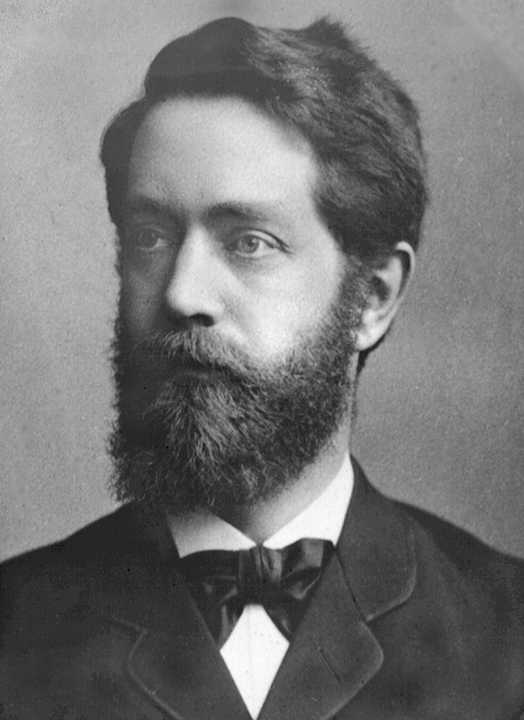
\includegraphics[width=\linewidth]{../../figures/portraits/felix-klein.jpg}\\
      {\scriptsize\color{gray}Felix Klein (1849--1925).}
    \end{column}
    \begin{column}{0.7\textwidth}
      Klein propose de distinguer les géométries non par leurs axiomes,
      mais par leurs \defi{transformations} : l'étude des propriétés
      d'une figure qui restent inchangées sous les transformations
      d'un certain groupe.
      \begin{itemize}
        \item Groupe des \textbf{isométries} : longueurs, angles, aires
          --- géométrie euclidienne du secondaire.
        \item Groupe des \textbf{similitudes} : angles et
          \emph{rapports} de longueurs --- figures semblables.
        \item Groupe des \textbf{transformations affines} : alignement,
          parallélisme, rapports sur une même droite.
        \item Toutes les déformations continues : propriétés
          topologiques seulement.
      \end{itemize}
    \end{column}
  \end{columns}
  \vspace{2pt}
  Plus le groupe est grand, moins on conserve de choses --- mais ce qui
  reste est plus profond. C'est cette hiérarchie qui organise le
  chapitre.
\end{frame}

% ═══════════════════════════════════════════════════════════════════════
\section{Qu'est-ce qu'une transformation du plan ?}
% ═══════════════════════════════════════════════════════════════════════

\begin{frame}{Le plan euclidien}
  On travaille dans le \defi{plan euclidien} $\Plan = \R^2$ : un
  ensemble de points, muni d'une distance $d(P,Q)$.
  \[
    P = (x,y) \qquad\text{ou}\qquad P = \col{x}{y} \in \R^2 .
  \]
  \vspace{6pt}
  Tout ce qui suit repose sur \textbf{une seule} définition.
\end{frame}

\begin{frame}{Définition 1.1 --- Transformation géométrique du plan}
  \begin{Enonce}{Définition 1.1 --- Transformation géométrique du plan}
    Une \defi{transformation géométrique} du plan est une
    \textbf{bijection} du plan dans lui-même : une fonction bijective
    $f : \Plan \longrightarrow \Plan$. On note $\Transf$ l'ensemble de
    toutes les transformations du plan.
  \end{Enonce}
  \FigBox[0.42\textheight]{%
    \begin{tikzpicture}[scale=0.95]
      \begin{scope}
        \draw[sectioncolor!50, thick, fill=steelblue4!8]
          (0,0) -- (4,0) -- (5,2.3) -- (1,2.3) -- cycle;
        \node[etiq, sectioncolor,above] at (0.55,2) {$\Plan$};
        \node[pt, label={[etiq]below:$P$}] (P) at (1.4,0.75) {};
        \node[pt, label={[etiq]below:$Q$}] (Q) at (2.6,1.5) {};
      \end{scope}
      \begin{scope}[xshift=6.6cm]
        \draw[firebrick3!50, thick, fill=firebrick3!8]
          (0,0) -- (4,0) -- (5,2.3) -- (1,2.3) -- cycle;
        \node[etiq, firebrick3,above] at (0.55,2) {$\Plan$};
        \node[ptim, label={[etiq]below:$f(P)$}] (Pp) at (2.9,0.6) {};
        \node[ptim, label={[etiq]above:$f(Q)$}] (Qp) at (1.7,1.7) {};
      \end{scope}
      \draw[fleche] (P) to[bend left=12] (Pp);
      \draw[fleche] (Q) to[bend left=12] (Qp);
      \node[etiq, sectioncolor] at (5.6,2.6) {$f$};
    \end{tikzpicture}}
  \begin{center}\small Figure 1.2\end{center}
\end{frame}

\begin{frame}{Décortiquer la définition}
  « Fonction » exige :
  \begin{itemize}
    \item[(i)] $f$ \textbf{partout définie} : chaque point $P$ a une image ;
    \item[(ii)] $f$ \textbf{univoque} : une seule image par point.
  \end{itemize}
  « Bijective » ajoute, \textbf{indépendamment} :
  \begin{itemize}
    \item[(iii)] \textbf{injectivité} : $P \neq Q \Rightarrow f(P) \neq f(Q)$ ;
    \item[(iv)] \textbf{surjectivité} : tout $Q$ possède un antécédent.
  \end{itemize}
  \vspace{6pt}
  \small Quatre conditions indépendantes : les exemples qui suivent
  montrent chacune de leurs violations possibles.
\end{frame}

\begin{frame}{Pour la classe 1.1 --- Trois mises en garde de vocabulaire}
  \begin{Classe}{Trois mises en garde de vocabulaire}
    \begin{enumerate}
      \item Si $Q = f(P)$ : $Q$ est l'\defi{image} de $P$, $P$ un
        \defi{antécédent} de $Q$.
      \item « $P$ s'est déplacé en $Q$ » est une façon de parler
        commode --- mais \textbf{les points ne bougent pas}. Une
        transformation est une \emph{correspondance}, pas un
        mouvement.
      \item Une transformation agit sur \textbf{tout} le plan, pas
        seulement sur la figure dessinée. « Faire tourner un
        triangle », c'est en réalité faire tourner le plan tout
        entier.
    \end{enumerate}
  \end{Classe}
\end{frame}

\begin{frame}{Exemples, et surtout contre-exemples}
  \small Rien ne clarifie mieux une définition que des objets qui n'y
  satisfont pas de justesse.
\end{frame}

\begin{frame}{Exemple 1.1 --- Une symétrie centrale}
  \begin{Enonce}{Exemple 1.1}
    \small Soit $M$ fixe. $f_1(P) = P'$, l'unique point tel que $M$
    soit le milieu de $[PP']$. \textbf{C'est une transformation} :
    chaque point a exactement une image, et chaque point est l'image
    d'exactement un point.
  \end{Enonce}
  \FigBox[0.42\textheight]{%
    \begin{tikzpicture}[scale=1.15]
      \node[pt, label={[etiq]below right:$M$}] (M) at (0,0) {};
      \node[pt, label={[etiq]above right:$P$}] (P) at (1.7,0.9) {};
      \node[ptim, label={[etiq]below left:$P'$}] (Pp) at (-1.7,-0.9) {};
      \draw[sectioncolor!45, thin] (P) -- (Pp);
      \draw[fig] (1.7,0.9) -- (2.3,-0.1) -- (0.9,-0.4) -- cycle;
      \draw[figim] (-1.7,-0.9) -- (-2.3,0.1) -- (-0.9,0.4) -- cycle;
    \end{tikzpicture}}
  \small C'est la \defi{symétrie centrale} de centre $M$ : cas
  particulier d'une homothétie de rapport négatif (section~3).
\end{frame}

\begin{frame}{Exemple 1.2 --- Un repliage du plan}
  \begin{Enonce}{Exemple 1.2}
    \small Soit $d$ fixe. $f_2$ laisse fixe le côté « nord » de $d$, et
    envoie le côté « sud » sur son réfléchi. C'est l'effet de replier
    une feuille sur $d$.
  \end{Enonce}
  \FigBox[0.38\textheight]{%
    \begin{tikzpicture}[scale=1.05]
      \draw[droite] (-2.2,0) -- (2.2,0) node[etiq, right, black] {$d$};
      \foreach \x/\y in {-1.4/1.1, -0.3/0.6, 1.2/0.4}
        {\node[pt] at (\x,\y) {};}
      \foreach \x/\y in {-1.4/-1.1, -0.3/-0.6, 1.2/-0.4}
        {\node[ptim] at (\x,\y) {};
         \draw[gray!60, thin, dotted, -{Stealth[length=1.6mm]}] (\x,\y) -- (\x,-\y);}
    \end{tikzpicture}}
  \textbf{Ce n'est PAS une transformation} : ni injective (deux
  antécédents au nord), ni surjective (rien n'atteint le sud).
\end{frame}

\begin{frame}{Exemple 1.3 --- L'arrondi au pixel près}
  \begin{Enonce}{Exemple 1.3}
    \small $f_3(x,y) = $ le point à coordonnées entières le plus
    proche. C'est ce que fait un écran en affichant une image sur sa
    grille de pixels.
  \end{Enonce}
  \FigBox[0.38\textheight]{%
    \begin{tikzpicture}[scale=0.95]
      \repere{-0.6}{3.6}{-0.6}{2.6}
      \foreach \x/\y in {1/1, 3/2}
        {\fill[firebrick3!18] (\x-0.5,\y-0.5) rectangle (\x+0.5,\y+0.5);
         \node[ptim] at (\x,\y) {};}
    \end{tikzpicture}}
  \textbf{Ce n'est PAS une transformation} : un carré entier s'écrase
  sur un point (pas injective), et les points non entiers ne sont
  jamais atteints (pas surjective).
\end{frame}

% ═══════════════════════════════════════════════════════════════════════
\section{Composer sans jamais sortir de l'ensemble}
% ═══════════════════════════════════════════════════════════════════════

\begin{frame}{Définition 1.2 --- Égalité et composition}
  \begin{Enonce}{Définition 1.2 --- Égalité et composition}
    Pour $f,g \in \Transf$ : $f = g$ si et seulement si $f(P) = g(P)$
    pour tout $P$. La \defi{composée} $f \circ g$ est définie par
    \[
      (f \circ g)(P) = f\bigl(g(P)\bigr).
    \]
  \end{Enonce}
  \vspace{6pt}
  \textbf{Attention à l'ordre} : dans $f \circ g$, c'est $g$ qui agit
  \emph{en premier}. Source d'erreurs constante --- et difficulté
  classique au secondaire.
  \vspace{4pt}

  \small La composée de deux transformations est encore une
  transformation (il suffit de vérifier les quatre conditions de la
  définition~1.1).
\end{frame}

\begin{frame}{Exemple 1.4 --- La composition n'est pas commutative}
  \small $r$ = rotation de $90°$ à l'origine ; $R$ = réflexion d'axe
  des $x$. Même motif, deux ordres de composition :
  \FigBox[0.46\textheight]{%
    \begin{tikzpicture}[scale=1.05]
      \begin{scope}
        \draw[quadrillage] (-1.2,-1.2) grid (1.2,1.2);
        \draw[axe] (-1.2,0) -- (1.35,0); \draw[axe] (0,-1.2) -- (0,1.35);
        \fill[fig] \motifF;
        \node[etiq, black] at (0,-1.45) {motif de départ};
      \end{scope}
      \begin{scope}[xshift=3.4cm]
        \draw[quadrillage] (-1.2,-1.2) grid (1.2,1.2);
        \draw[axe] (-1.2,0) -- (1.35,0); \draw[axe] (0,-1.2) -- (0,1.35);
        \begin{scope}[cm={0,1,-1,0,(0,0)}]
          \begin{scope}[cm={1,0,0,-1,(0,0)}]
            \fill[figim] \motifF;
          \end{scope}
        \end{scope}
        \node[etiq, black] at (0,-1.45) {$r \circ R$};
      \end{scope}
      \begin{scope}[xshift=6.8cm]
        \draw[quadrillage] (-1.2,-1.2) grid (1.2,1.2);
        \draw[axe] (-1.2,0) -- (1.35,0); \draw[axe] (0,-1.2) -- (0,1.35);
        \begin{scope}[cm={1,0,0,-1,(0,0)}]
          \begin{scope}[cm={0,1,-1,0,(0,0)}]
            \fill[figaux] \motifF;
          \end{scope}
        \end{scope}
        \node[etiq, black] at (0,-1.45) {$R \circ r$};
      \end{scope}
    \end{tikzpicture}}
  Les deux images sont symétriques par rapport à l'origine :
  $r \circ R \neq R \circ r$.
\end{frame}

\begin{frame}{Théorème 1.1 --- Propriétés de $(\Transf, \circ)$}
  \begin{Enonce}{Théorème 1.1 --- Propriétés de $(\Transf, \circ)$}
    \small Pour $f,g,h \in \Transf$ :
    \begin{enumerate}
      \item[(i)] \textbf{fermeture} : $f \circ g \in \Transf$ ;
      \item[(ii)] \textbf{associativité} : $(f\circ g)\circ h = f\circ(g\circ h)$ ;
      \item[(iii)] \textbf{identité} : $\mathrm{id} \in \Transf$,
        $f \circ \mathrm{id} = \mathrm{id} \circ f = f$ ;
      \item[(iv)] \textbf{inverse} : il existe $f^{-1}\in\Transf$ tel
        que $f\circ f^{-1} = f^{-1}\circ f = \mathrm{id}$.
    \end{enumerate}
    En général $f \circ g \neq g \circ f$.
  \end{Enonce}
  \begin{AuTableau}
    \small Idée : la fermeture se vérifie directement sur les 4
    conditions ; l'associativité vaut pour toute composition de
    fonctions ; l'inverse existe car $f$ est bijective, par
    définition.
  \end{AuTableau}
\end{frame}

\begin{frame}{Remarque 1.1 --- Inverser une composée}
  \begin{Rem}{Remarque 1.1 --- Inverser une composée}
    \[
      (f \circ g)^{-1} = g^{-1} \circ f^{-1} \qquad\text{(l'ordre s'inverse !)}
    \]
    Image classique : « mettre ses bas » puis « mettre ses souliers ».
    Pour défaire, on enlève d'abord les souliers.
  \end{Rem}
  \vspace{10pt}
  \begin{Rem}{Remarque 1.2 --- Le mot groupe}
    Fermeture, associativité, identité, inverse : les quatre axiomes
    d'un \defi{groupe}. On dira d'un ensemble de transformations qu'il
    est un \defi{sous-groupe} de $\Transf$ s'il est stable par
    composition et par inversion. (Théorie complète : MAT-2903.)
  \end{Rem}
\end{frame}

\begin{frame}{Figure 1.3 --- La hiérarchie des groupes de transformations}
  \FigBox[0.62\textheight]{%
    \begin{tikzpicture}[scale=1.05, every node/.style={font=\small}]
      \foreach \i/\lab/\prop in {%
         0/{$\Transf$ : toutes les transformations}/{aucun invariant métrique},
         1/{$\Aff$ : transformations affines}/{alignement, parallélisme},
         2/{$\Sim$ : similitudes}/{$+$ angles, rapports de longueurs},
         3/{$\Iso$ : isométries}/{$+$ longueurs, aires},
         4/{$\Iso^{+}$ : déplacements}/{$+$ orientation}}
        {\pgfmathsetmacro{\w}{9.4-1.35*\i}
         \pgfmathsetmacro{\y}{-0.95*\i}
         \draw[rounded corners=2pt, fill=steelblue4!\the\numexpr8+10*\i\relax,
               draw=sectioncolor!60]
           ({-\w/2},{\y-0.36}) rectangle ({\w/2},{\y+0.36});
         \node at (0,\y) {\lab};
         \node[anchor=west, font=\scriptsize, gray!80!black]
           at ({\w/2+0.25},\y) {\prop};}
    \end{tikzpicture}}
  \small Plus on descend, plus le groupe est petit, plus il conserve de
  propriétés. C'est la lecture « à la Klein » --- et c'est le plan du
  chapitre.
\end{frame}

\begin{frame}{Remarque 1.3 --- Où sont les applications affines non inversibles ?}
  \begin{Rem}{Remarque 1.3}
    \small Chaque famille de la figure 1.3 est emboîtée dans
    $\Transf$ : par définition, elle n'est faite que de
    \textbf{bijections}. Il existe pourtant des \emph{applications}
    affines non bijectives (ex. une projection) : elles ne préservent
    en général \textbf{ni l'alignement ni le parallélisme}, et ne
    figurent dans \emph{aucune} des familles de la figure --- n'étant
    pas bijectives, elles ne sont même pas dans $\Transf$.

    \vspace{4pt}
    \textbf{« Affine » n'implique pas l'inversibilité ; « transformation
    affine », si.}
  \end{Rem}
\end{frame}

% ═══════════════════════════════════════════════════════════════════════
\section{Les transformations affines}
% ═══════════════════════════════════════════════════════════════════════

\begin{frame}{Du plan géométrique au plan des coordonnées}
  \small Jusqu'ici, tout a été dit sans calcul (point de vue
  \emph{synthétique}). On choisit maintenant un repère : chaque point
  devient un couple de nombres, chaque transformation devient une
  formule (point de vue \emph{analytique}).
  \[
    d(P,Q) = \norme{P - Q} = \sqrt{(x_P-x_Q)^2 + (y_P-y_Q)^2}.
  \]
  \begin{Rem}{Remarque 1.4 --- Points ou vecteurs ?}
    \small On confond volontairement point $P$ et vecteur
    $\overrightarrow{OP}$ (même colonne de nombres) --- abus commode et
    universel en infographie. Cela explique pourquoi une translation
    n'est \textbf{pas} une application linéaire.
  \end{Rem}
\end{frame}

\begin{frame}{Définition 1.3 --- Application affine du plan}
  \begin{Enonce}{Définition 1.3 --- Application affine du plan}
    Une \defi{application affine} du plan est $w:\R^2\to\R^2$,
    \[
      w\col{x}{y} = \mat{a}{b}{c}{d}\col{x}{y} + \col{e}{f}
      = A\col{x}{y} + \vec{t}, \qquad a,b,c,d,e,f\in\R.
    \]
    $A$ : \defi{partie linéaire} ; $\vec t$ : \defi{partie translation}.
  \end{Enonce}
  \vspace{4pt}
  Une application affine = une application linéaire \textbf{suivie
  d'une translation}. Cette phrase anodine décrit exactement les
  translations, rotations, réflexions, homothéties, cisaillements ---
  et leurs compositions.
\end{frame}

\begin{frame}{Remarque 1.5 --- Pourquoi « affine » et non « linéaire » ?}
  \begin{Rem}{Remarque 1.5}
    Une application linéaire $T$ vérifie $T(\vec 0) = \vec 0$ : elle
    fixe l'origine. Une translation ne fixe \textbf{aucun} point : les
    translations ne sont donc pas linéaires. On ajoute le terme
    $\vec t$ précisément pour les inclure --- d'où « affine ».
  \end{Rem}
  \vspace{6pt}
  \small (Un tour de passe-passe --- les coordonnées homogènes ---
  permettra de récupérer la linéarité, au prix d'une dimension : voir
  section~5.)

  \vspace{10pt}
  \textbf{Vocabulaire fixé pour tout le chapitre :}
  \begin{itemize}
    \item \defi{application affine} : n'importe quelle fonction de
      cette forme, \emph{sans condition sur $A$} ;
    \item \defi{transformation affine} : une application affine
      \textbf{bijective}, i.e. un élément de $\Aff$.
  \end{itemize}
\end{frame}

\begin{frame}{Proposition 1.2 --- Inversibilité}
  \begin{Enonce}{Proposition 1.2 --- Inversibilité}
    \small Une application affine de partie linéaire $A$, translation
    $\vec t$, est bijective si et seulement si $\dete(A) \neq 0$. Alors
    \[
      w^{-1}\col{x}{y} = A^{-1}\col{x}{y} - A^{-1}\vec{t}.
    \]
  \end{Enonce}
  \begin{AuTableau}
    \small Idée : $\dete(A)\neq 0 \Leftrightarrow A$ inversible
    $\Leftrightarrow$ $A$ injective (algèbre linéaire) ; on vérifie
    directement que la formule proposée est une réciproque.
  \end{AuTableau}
  \vspace{6pt}
  \textbf{Conséquence.} Les applications affines inversibles forment un
  sous-groupe $\Aff$ de $\Transf$ : le \defi{groupe affine} du plan.
\end{frame}

\begin{frame}{Proposition 1.3 --- Ce qu'une transformation affine conserve}
  \begin{Enonce}{Proposition 1.3}
    \footnotesize Soit $w$ une transformation affine. Alors :
    \begin{enumerate}
      \item l'image d'une droite est une droite ;
      \item l'image d'une droite par l'origine passe par $(e,f)$ ;
      \item l'image de deux droites parallèles reste parallèle ;
      \item l'image d'un segment est un segment ; le milieu va sur le milieu ;
      \item plus généralement : $w$ préserve les rapports de longueurs
        \emph{sur une même droite} ;
      \item l'image d'un parallélogramme est un parallélogramme.
    \end{enumerate}
  \end{Enonce}
  \begin{AuTableau}
    \footnotesize Idée : écriture paramétrique d'une droite,
    $P + s\vec u$ ; $w(P+s\vec u) = w(P) + s(A\vec u)$, et $A\vec u \neq
    \vec 0$ car $A$ est inversible.
  \end{AuTableau}
\end{frame}

\begin{frame}{Remarque 1.6 --- Ce qu'elle ne conserve \emph{pas}}
  \begin{Rem}{Remarque 1.6}
    Une transformation affine ne préserve \textbf{en général} ni les
    longueurs, ni les angles, ni la perpendicularité, ni les rapports
    de longueurs entre deux directions différentes. Un carré peut
    devenir un parallélogramme quelconque ; un cercle devient une
    ellipse.
    \vspace{4pt}

    En revanche, elle multiplie \textbf{toutes} les aires par le même
    facteur (à venir).
  \end{Rem}
\end{frame}

\begin{frame}{Visualiser : l'image du carré unité}
  \small Le geste le plus utile du chapitre : pour comprendre une
  transformation, regarder ce qu'elle fait au carré unité
  $[0,1]\times[0,1]$. Les \textbf{colonnes de $A$} sont les images de
  $\vec e_1,\vec e_2$ : le carré devient le parallélogramme qu'elles
  engendrent.
  \FigBox[0.5\textheight]{%
    \begin{tikzpicture}[scale=1.0]
      \begin{scope}
        \repere{-0.6}{2.6}{-0.6}{2.6}
        \fill[fig] (0,0) rectangle (1,1);
        \draw[fleche] (0,0) -- (1,0) node[etiq, below right] {$\vec{e}_1$};
        \draw[fleche] (0,0) -- (0,1) node[etiq, above left] {$\vec{e}_2$};
        \node[etiq] at (1.3,-1.15) {le carré unité};
      \end{scope}
      \begin{scope}[xshift=5.2cm]
        \repere{-0.6}{2.6}{-0.6}{2.6}
        \fill[figim] (0,0) -- (1.5,0.4) -- (2.0,1.7) -- (0.5,1.3) -- cycle;
        \draw[fleche, firebrick3] (0,0) -- (1.5,0.4)
          node[etiq, below right] {$A\vec{e}_1 = \col{a}{c}$};
        \draw[fleche, firebrick3] (0,0) -- (0.5,1.3)
          node[etiq, above left] {$A\vec{e}_2 = \col{b}{d}$};
        \node[etiq] at (1.3,-1.15) {son image par $A$};
      \end{scope}
    \end{tikzpicture}}
  \begin{center}\small Figure 1.4\end{center}
\end{frame}

\begin{frame}{Définition 1.4 --- Orientation}
  \begin{Enonce}{Définition 1.4 --- Orientation d'une base, du plan}
    \small $(\vec u,\vec v)$ est \defi{directe} si l'on passe de $\vec
    u$ à $\vec v$, par le plus petit angle, dans le sens
    trigonométrique ; \defi{indirecte} sinon. $w$
    \defi{préserve l'orientation} si elle envoie toute base directe sur
    une base directe ; elle la \defi{renverse} sinon.
  \end{Enonce}
  \FigBox[0.36\textheight]{%
    \begin{tikzpicture}[scale=1.0]
      \begin{scope}
        \draw[fleche] (0,0) -- (1,0) node[etiq, below right] {$\vec u$};
        \draw[fleche] (0,0) -- (55:1) node[etiq, above] {$\vec v$};
        \draw[sectioncolor, thin, -{Stealth[length=1.6mm]}]
          (0.42,0) arc (0:55:0.42);
        \node[etiq] at (0.2,-0.75) {base directe};
      \end{scope}
      \begin{scope}[xshift=3.4cm]
        \draw[fleche] (0,0) -- (1,0) node[etiq, below right] {$\vec u$};
        \draw[fleche] (0,0) -- (-55:1) node[etiq, below right] {$\vec v$};
        \draw[sectioncolor, thin, -{Stealth[length=1.6mm]}]
          (0.42,0) arc (0:-55:0.42);
        \node[etiq] at (0.2,-1.05) {base indirecte};
      \end{scope}
    \end{tikzpicture}}
\end{frame}

\begin{frame}{Proposition 1.4 --- Aire et déterminant}
  \begin{Enonce}{Proposition 1.4 --- Aire et déterminant}
    Soit $w$ affine de partie linéaire $A$, et $D$ une région d'aire
    $S$. Alors $\Aire(w(D)) = \lvert \dete(A)\rvert \cdot S$. Si
    $\dete(A) \neq 0$ : $w$ préserve l'orientation si $\dete(A)>0$, la
    renverse si $\dete(A)<0$.
  \end{Enonce}
  \small (Admis --- relève du théorème du changement de variables.
  Intuition : vrai pour le carré unité par définition du déterminant,
  donc pour tout carré du quadrillage, donc pour toute région
  raisonnable.)
  \begin{Classe}{Le F est-il à l'endroit ?}
    \small Le signe du déterminant : $\dete(A)>0$, la figure se lit
    dans le même sens ; $\dete(A)<0$, elle est retournée comme dans un
    miroir. D'où l'usage d'un motif en « F » dans les figures : un F
    retourné se repère au premier coup d'œil.
  \end{Classe}
\end{frame}

\begin{frame}{Exemple 1.5 --- Image d'un rectangle}
  \small $w\col{x}{y} = \mat{1}{-1}{2}{0}\col{x}{y}+\col{-1}{1}$,
  $R=\intff{0}{2}\times\intff{0}{1}$. Il suffit de calculer l'image des
  4 sommets (prop.~1.3).
  \FigBox[0.42\textheight]{%
    \begin{tikzpicture}[scale=0.62]
      \begin{scope}
        \repere{-2.6}{2.6}{-0.6}{5.6}
        \fill[fig] (0,0) rectangle (2,1);
        \node[etiq] at (1,0.5) {$R$};
      \end{scope}
      \begin{scope}[xshift=7.6cm]
        \repere{-2.6}{2.6}{-0.6}{5.6}
        \fill[figim] (-1,1) -- (1,5) -- (0,5) -- (-2,1) -- cycle;
        \node[etiq, ptim, label={[etiq]below right:$(-1,1)$}] at (-1,1) {};
        \node[ptim, label={[etiq]right:$(1,5)$}] at (1,5) {};
        \node[etiq] at (-0.55,3) {$w(R)$};
      \end{scope}
    \end{tikzpicture}}
  Vérification par les aires : $\dete(A) = 2$, aire de $R$ = 2, donc
  aire de $w(R) = 4$ (confirmé).
\end{frame}

\begin{frame}{Exemple 1.6 --- Image d'un triangle}
  \small Même $w$. Triangle plein $A=(1,1)$, $B=(0,0)$, $C=(-1,1)$
  (isocèle) $\longmapsto$ triangle plein $(-1,3)$, $(-1,1)$, $(-3,-1)$
  (\textbf{pas} isocèle).

  \vspace{6pt}
  \textbf{Une transformation affine ne respecte pas les longueurs.}
\end{frame}

% ═══════════════════════════════════════════════════════════════════════
\section{Un catalogue d'applications affines}
% ═══════════════════════════════════════════════════════════════════════

\begin{frame}{Les briques du chapitre}
  \small On passe en revue les applications affines élémentaires ---
  toutes des transformations, sauf la dernière (la projection). Ce sont
  les briques : toute application linéaire inversible du plan s'obtient
  en les composant (théorème de décomposition, plus loin).

  \vspace{6pt}
  Convention de notation, valable pour tout le chapitre : rotations en
  $r$ minuscule, réflexions en $R$ majuscule. $r_\theta$ / $R_\theta$ :
  centrées à l'origine. $r_{M,\theta}$ / $R_d$ : centre ou axe précisé
  explicitement --- \textbf{un indice à deux éléments}.
\end{frame}

\subsection{Translations}
\begin{frame}{Définition 1.5 --- Translation}
  \begin{Enonce}{Définition 1.5 --- Translation}
    La \defi{translation} de vecteur $\vec t = \col{e}{f}$ est
    \[
      t_{\vec t}\col{x}{y} = \col{x}{y} + \col{e}{f}
      = \mat{1}{0}{0}{1}\col{x}{y} + \col{e}{f}.
    \]
  \end{Enonce}
  \vspace{6pt}
  \small Partie linéaire = identité : aires et orientation préservées
  --- première isométrie. Composer deux translations donne une
  translation, et \textbf{l'ordre n'y change rien} :
  $t_{\vec u}\circ t_{\vec v} = t_{\vec u+\vec v} = t_{\vec v}\circ t_{\vec u}$.
\end{frame}

\subsection{Homothéties}
\begin{frame}{Définition 1.6 --- Homothétie de centre l'origine}
  \begin{Enonce}{Définition 1.6}
    L'\defi{homothétie} de centre $\vec 0$, rapport $c\in\Rs$ :
    $h_c\col{x}{y} = \mat{c}{0}{0}{c}\col{x}{y}$. $0<c<1$ : contraction
    uniforme ; $c>1$ : dilatation uniforme ; $c<0$ : retourne la figure
    ($h_{-1}$ = symétrie centrale).
  \end{Enonce}
  \small $\dete(cI) = c^2 > 0$ : une homothétie ne renverse
  \textbf{jamais} l'orientation, même si $c<0$ --- excellent sujet de
  discussion en classe.
\end{frame}

\begin{frame}{Proposition 1.5 --- Homothétie de centre quelconque}
  \begin{Enonce}{Proposition 1.5}
    L'homothétie de centre $M=(h,k)$, rapport $c$ :
    $h_{M,c} = t_{\vec m}\circ h_c \circ t_{-\vec m}$,
    \[
      h_{M,c}\col{x}{y} = \col{cx+h(1-c)}{cy+k(1-c)}.
    \]
  \end{Enonce}
  \begin{AuTableau}
    \small Technique de la \textbf{conjugaison} (sert partout) : on
    ramène le centre à l'origine, on fait la transformation, on
    revient. $P\mapsto P-\vec m\mapsto c(P-\vec m)\mapsto c(P-\vec
    m)+\vec m$.
  \end{AuTableau}
\end{frame}

\begin{frame}{Pour la classe 1.3 --- Lire une formule du secondaire}
  \begin{Classe}{Lire une formule du secondaire}
    \small $(x,y)\mapsto(cx+h(1-c), cy+k(1-c))$ --- exactement la
    formule de 2\up{e} secondaire. Vue comme
    $t_{\vec m}\circ h_c\circ t_{-\vec m}$ : « je vais au centre,
    j'agrandis, je reviens » --- rien à retenir.
  \end{Classe}
\end{frame}

\subsection{Rotations}
\begin{frame}{Définition 1.7 --- Rotation de centre l'origine}
  \begin{Enonce}{Définition 1.7}
    La \defi{rotation} d'angle $\theta$, sens antihoraire, autour de
    l'origine :
    $r_\theta = \mat{\cos\theta}{-\sin\theta}{\sin\theta}{\cos\theta}$.
  \end{Enonce}
  \FigBox[0.42\textheight]{%
    \begin{tikzpicture}[scale=1.4]
      \repere{-1.35}{1.6}{-1.35}{1.6}
      \draw[gray!45, thin] (0,0) circle (1);
      \draw[fleche] (0,0) -- (1,0) node[etiq, below right] {$\vec{e}_1$};
      \draw[fleche] (0,0) -- (0,1) node[etiq, below left] {$\vec{e}_2$};
      \draw[fleche, firebrick3] (0,0) -- (37:1)
        node[etiq, right] {$\col{\cos\theta}{\sin\theta}$};
      \draw[fleche, firebrick3] (0,0) -- (127:1)
        node[etiq, above left] {$\col{-\sin\theta}{\cos\theta}$};
      \draw[firebrick3, thin] (0.42,0) arc (0:37:0.42);
      \node[etiq, firebrick3] at (20:0.62) {$\theta$};
      \draw[firebrick3, thin] (0,0.42) arc (90:127:0.42);
    \end{tikzpicture}}
  \begin{center}\small Figure 1.5. $\dete(r_\theta)=1$ : aires et
    orientation préservées.\end{center}
\end{frame}

\begin{frame}{Remarque 1.7 --- Un ou deux indices ?}
  \begin{Rem}{Remarque 1.7}
    Un indice \textbf{seul}, comme $r_\theta$ : centrée à
    \textbf{l'origine}. Dès que le centre n'est pas l'origine, on le
    place en \textbf{premier} indice : $r_{M,\theta}$ --- l'indice
    porte alors sur \emph{deux} objets, jamais sur l'angle seul. Même
    lecture pour $h_c$ / $h_{M,c}$ et $R_\theta$ / $R_d$.
  \end{Rem}
  \[
    r_{M,\theta}\col{x}{y}
      = r_\theta\left(\col{x}{y} - \vec{m}\right) + \vec{m}
      = r_\theta\col{x}{y} + (I - r_\theta)\,\vec{m}
      \qquad\text{(conjugaison, encore.)}
  \]
\end{frame}

\begin{frame}{Proposition 1.6 --- Composer deux rotations de même centre}
  \begin{Enonce}{Proposition 1.6}
    Pour $M$ quelconque :
    $r_{M,\alpha}\,r_{M,\beta} = r_{M,\alpha+\beta} = r_{M,\beta}\,r_{M,\alpha}$,
    et $r_{M,\theta}^{-1} = r_{M,-\theta}$.
  \end{Enonce}
  \begin{AuTableau}
    \small Idée : cas $M=\vec 0$ par produit matriciel (les formules
    d'addition d'angles apparaissent) ; cas général par conjugaison,
    ramené au premier cas.
  \end{AuTableau}
  \begin{Classe}{Un cadeau pour la classe}
    \small La démonstration (cas $M=\vec 0$) est une preuve de
    $\cos(\alpha+\beta)=\cos\alpha\cos\beta-\sin\alpha\sin\beta$ et
    $\sin(\alpha+\beta)=\sin\alpha\cos\beta+\cos\alpha\sin\beta$ --- la
    plus courte qui soit, et elle explique \emph{pourquoi} : reflet
    d'un produit de matrices. À garder pour la 5\up{e} secondaire.
  \end{Classe}
\end{frame}

\subsection{Réflexions}
\begin{frame}{Définition 1.8 --- Réflexions}
  \begin{Enonce}{Définition 1.8 --- Réflexions par rapport aux axes}
    $H = \mat{1}{0}{0}{-1}$ (axe des $x$), $V=\mat{-1}{0}{0}{1}$ (axe
    des $y$).
  \end{Enonce}
  Plus généralement, réflexion d'axe passant par l'origine, angle
  $\theta$ avec l'axe des $x$ :
  \[
    R_\theta = \mat{\cos 2\theta}{\sin 2\theta}{\sin 2\theta}{-\cos 2\theta}.
  \]
  \small $\dete(R_\theta) = -1$ : une réflexion renverse toujours
  l'orientation (intuition du miroir). $\theta=0$ : $H$. $\theta=\pi/4$ :
  réflexion d'axe $y=x$, matrice $\mat{0}{1}{1}{0}$ (échange les
  coordonnées).
\end{frame}

\begin{frame}{Remarque 1.8 --- L'angle double}
  \begin{Rem}{Remarque 1.8}
    Le $2\theta$ n'est \textbf{pas} une coquille : faire tourner le
    \emph{miroir} de $\theta$ fait tourner l'\emph{image} de
    $2\theta$. Même phénomène : la composée de deux réflexions d'axes
    sécants est une rotation d'angle \textbf{double} de l'angle des
    axes (théorème~1.13, plus loin) --- l'un des plus beaux résultats
    à faire découvrir au secondaire.
  \end{Rem}
\end{frame}

\subsection{Cisaillements et contractions non uniformes}
\begin{frame}{Définition 1.9 --- Cisaillement}
  \begin{Enonce}{Définition 1.9}
    \defi{Cisaillement horizontal} de rapport $m$ : $\mat{1}{m}{0}{1}$.
    \defi{Cisaillement vertical} de rapport $m$ : $\mat{1}{0}{m}{1}$.
  \end{Enonce}
  \small Le cisaillement horizontal laisse fixe l'axe des $x$ et fait
  glisser chaque droite horizontale proportionnellement à sa hauteur ---
  un paquet de cartes qui penche. $\dete = 1$ : \textbf{un cisaillement
  conserve les aires}, en déformant complètement angles et longueurs.
  \begin{Classe}{Le cisaillement et l'aire du parallélogramme}
    \small « Aire = base $\times$ hauteur » : un cisaillement bien
    choisi transforme le parallélogramme en un rectangle de même base
    et hauteur, en conservant l'aire. C'est exactement ce que l'on fait
    au secondaire en découpant un triangle et en le déplaçant --- sans
    savoir qu'on vient de faire un cisaillement.
  \end{Classe}
\end{frame}

\begin{frame}{Définition 1.10 --- Contraction non uniforme}
  \begin{Enonce}{Définition 1.10}
    Application linéaire $\mat{a}{0}{0}{b}$, $0<a<1$, $0<b<1$.
  \end{Enonce}
  \small Si $a\neq b$ : contracte davantage dans une direction ---
  un cercle devient une ellipse. Avec $a>1$, $0<b<1$ : dilatation
  horizontale et contraction verticale. Essentielles dans la
  construction des fractales \emph{auto-affines} (fougère de Barnsley).
\end{frame}

\begin{frame}{Figure 1.6 --- Le catalogue en images}
  \FigBox[0.66\textheight]{%
    \begin{tikzpicture}[scale=0.72]
      \begin{scope}[shift={(0,0)}]
        \draw[quadrillage] (-1.25,-1.25) grid (1.25,1.25);
        \draw[axe] (-1.25,0) -- (1.4,0);
        \draw[axe] (0,-1.25) -- (0,1.4);
        \draw[steelblue4!55, thin] \motifF;
        \begin{scope}[cm={1,0,0,1,(-0.9,-0.6)}]
          \fill[figim] \motifF;
        \end{scope}
        \node[etiq, black, align=center] at (0,-1.72)
          {translation\\$\vec{t}=(-0{,}9\,;-0{,}6)$};
      \end{scope}
      \begin{scope}[shift={(3.5,0)}]
        \draw[quadrillage] (-1.25,-1.25) grid (1.25,1.25);
        \draw[axe] (-1.25,0) -- (1.4,0);
        \draw[axe] (0,-1.25) -- (0,1.4);
        \draw[steelblue4!55, thin] \motifF;
        \begin{scope}[cm={0,1,-1,0,(0,0)}]
          \fill[figim] \motifF;
        \end{scope}
        \node[etiq, black, align=center] at (0,-1.72)
          {rotation\\$\theta = 90°$};
      \end{scope}
      \begin{scope}[shift={(7,0)}]
        \draw[quadrillage] (-1.25,-1.25) grid (1.25,1.25);
        \draw[axe] (-1.25,0) -- (1.4,0);
        \draw[axe] (0,-1.25) -- (0,1.4);
        \draw[steelblue4!55, thin] \motifF;
        \begin{scope}[cm={1,0,0,-1,(0,0)}]
          \fill[figim] \motifF;
        \end{scope}
        \node[etiq, black, align=center] at (0,-1.72)
          {réflexion\\d'axe $Ox$};
      \end{scope}
      \begin{scope}[shift={(0,-4.3)}]
        \draw[quadrillage] (-1.25,-1.25) grid (1.25,1.25);
        \draw[axe] (-1.25,0) -- (1.4,0);
        \draw[axe] (0,-1.25) -- (0,1.4);
        \draw[steelblue4!55, thin] \motifF;
        \begin{scope}[cm={0.55,0,0,0.55,(0,0)}]
          \fill[figim] \motifF;
        \end{scope}
        \node[etiq, black, align=center] at (0,-1.72)
          {homothétie\\$c = 0{,}55$};
      \end{scope}
      \begin{scope}[shift={(3.5,-4.3)}]
        \draw[quadrillage] (-1.25,-1.25) grid (1.25,1.25);
        \draw[axe] (-1.25,0) -- (1.4,0);
        \draw[axe] (0,-1.25) -- (0,1.4);
        \draw[steelblue4!55, thin] \motifF;
        \begin{scope}[cm={1,0.8,0,1,(0,0)}]
          \fill[figim] \motifF;
        \end{scope}
        \node[etiq, black, align=center] at (0,-1.72)
          {cisaillement\\vertical, $m=0{,}8$};
      \end{scope}
      \begin{scope}[shift={(7,-4.3)}]
        \draw[quadrillage] (-1.25,-1.25) grid (1.25,1.25);
        \draw[axe] (-1.25,0) -- (1.4,0);
        \draw[axe] (0,-1.25) -- (0,1.4);
        \draw[steelblue4!55, thin] \motifF;
        \begin{scope}[cm={0.5,0,0,0.85,(0,0)}]
          \fill[figim] \motifF;
        \end{scope}
        \node[etiq, black, align=center] at (0,-1.72)
          {contraction\\non uniforme};
      \end{scope}
    \end{tikzpicture}}
  \begin{center}\small Le « F » : seule la réflexion renverse
  l'orientation.\end{center}
\end{frame}

\begin{frame}{Table 1.1 --- Récapitulatif}
  \small
  \begin{center}
  \begin{tabular}{llcc}
    \toprule
    Transformation & Matrice $A$ & $\dete(A)$ & Isométrie ? \\
    \midrule
    Translation & $I$ & $1$ & oui \\[4pt]
    Rotation d'angle $\theta$
      & $\mat{\cos\theta}{-\sin\theta}{\sin\theta}{\cos\theta}$
      & $1$ & oui \\[10pt]
    Réflexion d'axe $\theta$
      & $\mat{\cos 2\theta}{\sin 2\theta}{\sin 2\theta}{-\cos 2\theta}$
      & $-1$ & oui \\[10pt]
    Homothétie de rapport $c$
      & $\mat{c}{0}{0}{c}$ & $c^2$ & si $\lvert c\rvert = 1$ \\[10pt]
    Cisaillement de rapport $m$
      & $\mat{1}{m}{0}{1}$ & $1$ & non (sauf $m=0$) \\[10pt]
    Contraction non uniforme
      & $\mat{a}{0}{0}{b}$ & $ab$ & non (sauf $\lvert a\rvert=\lvert b\rvert=1$) \\[10pt]
    Projection sur $y=x$
      & $\tfrac12\mat{1}{1}{1}{1}$ & $0$ & non (non inversible) \\
    \bottomrule
  \end{tabular}
  \end{center}
\end{frame}

\subsection{Le cas non inversible}
\begin{frame}{Le cas non inversible}
  \small On considère parfois des applications affines qui ne sont pas
  des transformations : $\dete(A) = 0$. Tout le plan est alors écrasé
  sur une droite ($A\neq 0$) ou un point ($A=0$).

  \begin{Enonce}{Exemple 1.7 --- La projection orthogonale sur $y=x$}
    \small $p\col{x}{y} = \tfrac{x+y}{2}\col{1}{1}
      = \tfrac12\mat{1}{1}{1}{1}\col{x}{y}$. $\dete = 0$ : toutes les
      aires sont écrasées à zéro. Notez $p\circ p = p$.
  \end{Enonce}
  \FigBox[0.32\textheight]{%
    \begin{tikzpicture}[scale=1.15]
      \repere{-1.4}{2.4}{-1.4}{2.4}
      \draw[droite] (-1.3,-1.3) -- (2.3,2.3) node[etiq, right, black] {$y=x$};
      \fill[fig] \motifF;
      \draw[firebrick3, ultra thick] (0,0) -- (0.875,0.875);
      \foreach \x/\y in {0/1, 0.75/1, 0.3/0, 0.6/0.55}
        {\draw[gray!70, thin, dotted] (\x,\y) -- ({(\x+\y)/2},{(\x+\y)/2});
         \node[pt, inner sep=0.7pt] at (\x,\y) {};
         \node[ptim, inner sep=0.7pt] at ({(\x+\y)/2},{(\x+\y)/2}) {};}
    \end{tikzpicture}}
  \begin{center}\small Figure 1.7 --- Le motif tout entier écrasé sur un
  segment. Pas une transformation du plan.\end{center}
\end{frame}

\subsection{Le théorème de décomposition}
\begin{frame}{Théorème 1.7 --- Décomposition}
  \begin{Enonce}{Théorème 1.7 --- Décomposition des applications linéaires}
    Une application linéaire de $\R^2$ est inversible si et seulement
    si elle est une composition d'homothéties, de rotations, de
    réflexions, de cisaillements et de contractions/dilatations non
    uniformes.
  \end{Enonce}
  \small C'est la version géométrique d'un fait d'algèbre linéaire :
  toute matrice inversible est un produit de matrices élémentaires.
  Cisaillements $\leftrightarrow$ addition d'un multiple d'une ligne à
  une autre ; contractions non uniformes $\leftrightarrow$
  multiplication d'une ligne par un scalaire ; réflexion d'axe $y=x$
  $\leftrightarrow$ échange de deux lignes. \textbf{Gauss--Jordan est
  une décomposition géométrique.}
  \begin{Rem}{Remarque 1.9 --- Deux décompositions modernes}
    \footnotesize \emph{Polaire} : $A=QS$ (rotation/réflexion, puis
    déformation symétrique positive). \emph{SVD} : $A=U\Sigma V^\top$
    --- « une rotation, un étirement selon les axes, une rotation ».
    Explique pourquoi un cercle devient toujours une ellipse.
  \end{Rem}
\end{frame}

% ═══════════════════════════════════════════════════════════════════════
\section{Coordonnées homogènes : le tour de passe-passe de l'infographie}
% ═══════════════════════════════════════════════════════════════════════

\begin{frame}{Le problème}
  \small Composer deux applications affines est pénible :
  \[
    (w_2\circ w_1)\col{x}{y} = (A_2A_1)\col{x}{y} + (A_2\vec t_1+\vec t_2)
  \]
  --- une règle pour $A$, une autre pour $\vec t$. Sur une carte
  graphique qui compose des milliers de transformations par image, ce
  n'est pas acceptable.

  \vspace{6pt}
  \textbf{L'astuce} : plonger le plan dans $\R^3$, à la hauteur $z=1$ :
  $(x,y) \mapsto (x,y,1)$.
  \[
    \begin{pmatrix} a & b & e\\ c & d & f\\ 0 & 0 & 1\end{pmatrix}
    \coliii{x}{y}{1} = \coliii{ax+by+e}{cx+dy+f}{1}.
  \]
  La translation devient une multiplication matricielle : l'affine est
  redevenue linéaire, une dimension plus haut.
\end{frame}

\begin{frame}{Figure 1.8 --- Points et vecteurs, en coordonnées homogènes}
  \FigBox[0.5\textheight]{%
    \begin{tikzpicture}[scale=1.1]
      \draw[sectioncolor!45, fill=steelblue4!10]
        (0,1.6) -- (4.2,1.6) -- (5.4,2.9) -- (1.2,2.9) -- cycle;
      \node[etiq, sectioncolor] at (5.05,2.55) {$z=1$};
      \draw[gray!55, fill=gray!8]
        (0,-0.5) -- (4.2,-0.5) -- (5.4,0.8) -- (1.2,0.8) -- cycle;
      \node[etiq, gray!70!black] at (5.05,0.45) {$z=0$};
      \node[pt] (O) at (2.1,0.15) {};
      \node[etiq] at (1.75,-0.05) {$(0,0,0)$};
      \node[pt, label={[etiq]above right:$(x,y,1)$}] (P) at (2.85,2.1) {};
      \draw[fleche, dashed] (O) -- (P);
      \node[etiq, align=left, sectioncolor] at (7.9,2.1)
        {le plan des points,\\relevé à la hauteur~1};
      \node[etiq, align=left, gray!70!black] at (7.9,0.15)
        {le plan des vecteurs\\(directions)};
    \end{tikzpicture}}
  \small Les points vivent à $z=1$, les vecteurs (directions) à $z=0$.
  La distinction point/vecteur redevient visible.
\end{frame}

\begin{frame}{Les avantages}
  \begin{enumerate}
    \item \textbf{Composer, c'est multiplier.} La matrice de
      $w_2\circ w_1$ est le produit des deux matrices $3\times3$, dans
      cet ordre. Une seule règle au lieu de deux.
    \item \textbf{Inverser, c'est inverser.} La matrice de $w^{-1}$ est
      l'inverse de la matrice $3\times3$.
    \item \textbf{La distinction point/vecteur revient.} Point =
      $(x,y,1)$ ; vecteur = $(x,y,0)$. La différence de deux points
      donne un vecteur ; une translation ne change pas un vecteur.
    \item \textbf{On peut aller plus loin.} En autorisant la troisième
      ligne à différer de $(0,0,1)$ : transformations
      \emph{projectives}, celles de la perspective en 3D.
  \end{enumerate}
\end{frame}

\begin{frame}{Exemple 1.8 --- Faire pivoter, puis glisser, une maison}
  \small Maison de sommets $(0,0),(2,0),(2,1{,}4),(1,2{,}2),(0,1{,}4)$.
  $r$ = rotation $\pi/2$, puis $t$ = translation $(3,1)$ :
  \[
    M_r = \begin{pmatrix} 0&-1&0\\ 1&0&0\\ 0&0&1\end{pmatrix},\quad
    M_t = \begin{pmatrix} 1&0&3\\ 0&1&1\\ 0&0&1\end{pmatrix},\quad
    M_tM_r = \begin{pmatrix} 0&-1&3\\ 1&0&1\\ 0&0&1\end{pmatrix}.
  \]
  Coin $(2,0) = (2,0,1)$ : $M_tM_r\coliii{2}{0}{1} = \coliii{3}{3}{1}$ ---
  identique au calcul affine direct
  $r_{\pi/2}\col{2}{0}+\col{3}{1}$, en une seule multiplication.
  \FigBox[0.32\textheight]{%
    \begin{tikzpicture}[scale=0.85]
      \repere{-0.6}{3.6}{-0.6}{3.6}
      \fill[fig] (0,0) -- (2,0) -- (2,1.4) -- (1,2.2) -- (0,1.4) -- cycle;
      \fill[figim] (3,1) -- (3,3) -- (1.6,3) -- (0.8,2) -- (1.6,1) -- cycle;
      \node[etiq] at (0.6,-0.95) {maison};
      \node[etiq] at (2.9,3.75) {$(t \circ r)(\text{maison})$};
    \end{tikzpicture}}
\end{frame}

\begin{frame}{Attention à l'ordre, encore}
  \small En composant dans l'autre ordre, $r\circ t$ (glisser, puis
  tourner) :
  \[
    M_rM_t = \begin{pmatrix} 0&-1&0\\ 1&0&0\\ 0&0&1\end{pmatrix}
    \begin{pmatrix} 1&0&3\\ 0&1&1\\ 0&0&1\end{pmatrix}
    = \begin{pmatrix} 0&-1&-1\\ 1&0&3\\ 0&0&1\end{pmatrix}
    \neq M_tM_r.
  \]
  La composition en coordonnées homogènes n'échappe pas à la remarque
  1.1.

  \begin{Rem}{Remarque 1.10 --- Où c'est réellement utilisé}
    \small Un personnage qui bouge dans un jeu vidéo, un bras de robot,
    une image redressée, une carte qui pivote : des produits de
    matrices $3\times 3$ calculés par millions et par seconde ---
    l'application des mathématiques du secondaire la plus omniprésente
    et la moins connue des élèves.
  \end{Rem}
\end{frame}

% ═══════════════════════════════════════════════════════════════════════
\section{Isométries et similitudes}
% ═══════════════════════════════════════════════════════════════════════

\begin{frame}{On descend d'un cran dans la hiérarchie}
  \small Parmi les transformations affines, celles qui intéressent le
  secondaire sont celles qui respectent la \emph{forme} des figures.

  \begin{Enonce}{Définition 1.11 --- Similitude, isométrie, contraction}
    $w$ affine est une \defi{similitude} de rapport $k>0$ si
    \[
      \norme{w(P)-w(Q)} = k\,\norme{P-Q} \qquad \forall P,Q.
    \]
    $k=1$ : \defi{isométrie}. $0<k<1$ : \defi{contraction}.
  \end{Enonce}
  \small C'est la définition de « figures semblables » du secondaire,
  énoncée comme propriété de la \emph{transformation}, non d'un couple
  de figures.
\end{frame}

\begin{frame}{Propositions 1.8 et 1.9}
  \begin{Enonce}{Proposition 1.8 --- Il suffit de regarder la partie linéaire}
    \small $w$ affine de partie linéaire $A$ est une similitude de
    rapport $k$ ssi $\col{x}{y}\mapsto A\col{x}{y}$ en est une, même
    rapport. (La translation disparaît dans la différence
    $w(P)-w(Q)$.)
  \end{Enonce}
  \begin{Enonce}{Proposition 1.9 --- Une composition de similitudes est une similitude}
    \small $w_1,w_2$ similitudes de rapports $k_1,k_2$
    $\Rightarrow$ $w_2\circ w_1$ similitude de rapport $k_1k_2$.
  \end{Enonce}
  \vspace{4pt}
  \textbf{Conséquence.} Les similitudes forment un sous-groupe $\Sim$
  de $\Aff$, les isométries un sous-groupe $\Iso$ de $\Sim$ : la figure
  1.3 est maintenant justifiée.
\end{frame}

\subsection{L'anatomie des similitudes}
\begin{frame}{L'anatomie des similitudes}
  \small Homothéties, rotations, réflexions, translations sont des
  similitudes, donc toutes leurs compositions aussi. On \textbf{admet}
  la réciproque : ce sont les seules --- la partie linéaire d'une
  similitude de rapport $k$ est toujours $k\,r_\theta$ (directe) ou
  $k\,R_\theta$ (indirecte), pour un certain $\theta$. (Démonstration
  complète hors cadre du cours.)
\end{frame}

\begin{frame}{Propositions 1.10 et 1.11}
  \begin{Enonce}{Proposition 1.10 --- Déterminant d'une similitude}
    \small $w$ similitude de rapport $k$, partie linéaire $A$ :
    $\dete(A) = k^2$ ou $-k^2$. Donc $\lvert\dete(A)\rvert = k^2$, et
    $w$ est une contraction ssi $\lvert\dete(A)\rvert < 1$.
  \end{Enonce}
  \begin{Enonce}{Proposition 1.11 --- Aires et rapport de similitude}
    Si $w$ est une similitude de rapport $k$ et $D$ une région du
    plan : $\Aire(w(D)) = k^2\,\Aire(D)$.
  \end{Enonce}
  \begin{Classe}{Le fameux $k^2$}
    \small « Si on double les dimensions, l'aire $\times 4$ » --- l'un
    des résultats les plus mal compris du secondaire. Deux preuves : le
    déterminant (prop.~1.4), ou le fait qu'une aire est un produit de
    deux longueurs, chacune $\times k$. Dimension 3 : $k^3$ pour les
    volumes.
  \end{Classe}
\end{frame}

\begin{frame}{Exemple 1.9 --- Reconnaître une similitude}
  \small $A=\mat{0{,}8}{0}{a}{0{,}6}$ n'est \textbf{jamais} une
  similitude ($\norme{A\vec e_1}\geq 0{,}8 \neq 0{,}6=\norme{A\vec
  e_2}$, contradiction).

  \vspace{6pt}
  $A=\mat{0{,}5}{\alpha}{\beta}{0{,}5}$ : similitude pour
  $\alpha=\beta=0$ (homothétie $\tfrac12$) et pour
  $\alpha=\tfrac{\sqrt3}2,\beta=-\tfrac{\sqrt3}2$ --- on reconnaît la
  matrice $r_{-\pi/3}$ : \textbf{c'est même une isométrie} ($k=1$).
\end{frame}

\subsection{Classification des isométries du plan}
\begin{frame}{Théorème 1.12 --- Les quatre isométries du plan}
  \begin{Enonce}{Théorème 1.12 (admis sans démonstration)}
    \small Toute isométrie du plan est :
    \begin{enumerate}
      \item une \defi{translation} (identité incluse) ;
      \item une \defi{rotation} autour d'un point ;
      \item une \defi{réflexion} par rapport à une droite ;
      \item une \defi{réflexion glissée} : réflexion suivie d'une
        translation parallèle à l'axe.
    \end{enumerate}
  \end{Enonce}
\end{frame}

\begin{frame}{Table 1.2 --- Les isométries, résumé}
  \begin{center}
  \begin{tabular}{llll}
    \toprule
    Isométrie & $\dete(A)$ & Points fixes & Nom au secondaire\\
    \midrule
    Identité         & $+1$ & tout le plan  & --- \\
    Translation      & $+1$ & aucun         & translation \\
    Rotation         & $+1$ & un seul point & rotation \\
    Réflexion        & $-1$ & une droite    & réflexion \\
    Réflexion glissée & $-1$ & aucun         & (absente du programme) \\
    \bottomrule
  \end{tabular}
  \end{center}
\end{frame}

\begin{frame}{Pour la classe 1.7 --- La grande absente}
  \begin{Classe}{La grande absente}
    \small La réflexion glissée ne figure pas au programme québécois.
    Elle explique les traces de pas dans la neige, la disposition des
    feuilles, plusieurs frises. La liste « translation, rotation,
    réflexion » que retiennent les élèves est \textbf{incomplète} :
    composer une réflexion et une translation donne, en général,
    quelque chose qui n'est aucune des trois.
  \end{Classe}
  \FigBox[0.3\textheight]{%
    \begin{tikzpicture}[scale=0.85]
      \draw[droite] (-0.5,0) -- (8.2,0);
      \foreach \i in {0,1,2,3}{
        \begin{scope}[shift={(2*\i,0)}, scale=0.55]
          \fill[fig] \motifF;
        \end{scope}
        \begin{scope}[shift={(2*\i+1,0)}, scale=0.55, yscale=-1]
          \fill[figim] \motifF;
        \end{scope}}
      \node[etiq, right] at (8.3,0) {axe};
    \end{tikzpicture}}
  \begin{center}\small Figure 1.9 --- Une frise engendrée par une
  réflexion glissée.\end{center}
\end{frame}

\subsection{Tout se ramène aux réflexions}
\begin{frame}{Théorème 1.13 --- Composée de deux réflexions}
  \begin{Enonce}{Théorème 1.13}
    \small Soient $d_1,d_2$, $R_1,R_2$ les réflexions correspondantes.
    \begin{enumerate}
      \item Si $d_1\parallel d_2$ : $R_2\circ R_1$ = translation de
        vecteur $2\vec v$, $\vec v$ perpendiculaire de $d_1$ à $d_2$.
      \item Si $d_1,d_2$ se coupent en $M$, angle $\varphi$ :
        $R_2\circ R_1$ = rotation de centre $M$, angle $2\varphi$.
    \end{enumerate}
  \end{Enonce}
  \FigBox[0.4\textheight]{%
    \begin{tikzpicture}[scale=1.25]
      \draw[droite] (-1.8,0) -- (1.8,0) node[etiq, right, black] {$d_1$};
      \draw[droite] (35:-1.8) -- (35:1.8) node[etiq, right, black] {$d_2$};
      \node[pt, label={[etiq]below left:$M$}] at (0,0) {};
      \draw[sectioncolor, thin] (0.6,0) arc (0:35:0.6);
      \node[etiq, sectioncolor] at (17:0.82) {$\varphi$};
      \begin{scope}[shift={(0.75,0.25)}, scale=0.5]
        \fill[fig] \motifF;
      \end{scope}
      \begin{scope}[cm={1,0,0,-1,(0,0)}]
        \begin{scope}[shift={(0.75,0.25)}, scale=0.5]
          \fill[figaux] \motifF;
        \end{scope}
      \end{scope}
      \begin{scope}[rotate=70]
        \begin{scope}[shift={(0.75,0.25)}, scale=0.5]
          \fill[figim] \motifF;
        \end{scope}
      \end{scope}
      \draw[-{Stealth[length=2mm]}, firebrick3, thick]
        (1.35,0.75) arc (25:95:1.5);
      \node[etiq, firebrick3] at (60:1.85) {$2\varphi$};
    \end{tikzpicture}}
  \begin{center}\small Figure 1.10\end{center}
\end{frame}

\begin{frame}{Corollaire 1.14, et une leçon de didactique}
  \begin{AuTableau}[Idée de la démonstration --- au tableau]
    \small Cas $2$ : quitte à translater, $M=\vec 0$ ; par
    $R_{\alpha+\varphi}R_\alpha$, développement trigonométrique
    $\Rightarrow r_{2\varphi}$.
  \end{AuTableau}
  \begin{Enonce}{Corollaire 1.14 --- Trois réflexions suffisent}
    Toute isométrie du plan est la composée d'au plus \textbf{trois}
    réflexions.
  \end{Enonce}
  \begin{Classe}{Une leçon de didactique}
    \small La réflexion n'est pas une transformation « parmi
    d'autres » : c'est \emph{la} transformation fondamentale, qui
    engendre toutes les autres. On peut faire vivre ce résultat avec
    deux miroirs, ou deux pliages successifs : les élèves découvrent
    expérimentalement que deux réflexions donnent une rotation d'angle
    double de l'angle entre les plis.
  \end{Classe}
\end{frame}

% ═══════════════════════════════════════════════════════════════════════
\section{Déterminer une transformation à partir de points}
% ═══════════════════════════════════════════════════════════════════════

\begin{frame}{La question inverse}
  \small Jusqu'ici : « voici une transformation, que fait-elle à cette
  figure ? ». Maintenant, la question qui se pose \textbf{en pratique} :
  « voici une figure et son image, quelle transformation les relie ? »
  --- le problème que résout un logiciel de retouche photo, ou de
  reconnaissance de formes.
\end{frame}

\begin{frame}{Théorème 1.15 --- Trois points suffisent}
  \begin{Enonce}{Théorème 1.15}
    \small $P_1,P_2,P_3$ \textbf{non alignés}, et $Q_1,Q_2,Q_3$
    quelconques. Il existe une \textbf{unique} application affine $w$
    telle que $w(P_i)=Q_i$, $i=1,2,3$.
  \end{Enonce}
  \small Surnommée \defi{méthode du bulldozer} : on écrit toutes les
  conditions et on pousse tout dans un système linéaire.
  \begin{AuTableau}
    \small Idée : le système à 6 inconnues $(a,b,c,d,e,f)$ se
    \textbf{découple} en deux systèmes $3\times 3$ de même matrice
    \[
      M = \begin{pmatrix} x_1&y_1&1\\x_2&y_2&1\\x_3&y_3&1\end{pmatrix},
      \qquad \dete(M) = 2\cdot\text{aire orientée}(P_1P_2P_3) \neq 0.
    \]
  \end{AuTableau}
\end{frame}

\begin{frame}{Remarque 1.11 --- Une écriture plus compacte}
  \begin{Rem}{Remarque 1.11}
    \small En coordonnées homogènes, tout tient sur une ligne. Avec
    $\widetilde P,\widetilde Q$ les matrices $3\times3$ des points
    (en colonnes, ligne du bas = 1) :
    \[
      \widetilde W = \widetilde Q\,\widetilde P^{-1}.
    \]
    C'est la formule qu'implémentent les bibliothèques d'infographie.
  \end{Rem}
\end{frame}

\begin{frame}{Exemple 1.10 --- Le problème des deux triangles}
  \small $A=(-11,3)$, $B=(1,12)$, $C=(-1,14)$
  $\longmapsto$ $P=(90,-68)$, $Q=(69,-53)$, $R=(83,-59)$.
  \[
    w\col{x}{y} = \mat{-4}{3}{2}{-1}\col{x}{y} + \col{37}{-43}.
  \]
  $\dete(A)=-2$ : renverse l'orientation, double les aires. Ni une
  isométrie, ni une similitude ($A^\top A$ n'est pas multiple de $I$).
  \FigBox[0.36\textheight]{%
    \begin{tikzpicture}[scale=0.2]
      \draw[quadrillage] (-12,-1) grid (3,16);
      \draw[axe] (-12,0) -- (3.6,0) node[etiq, below] {$x$};
      \draw[axe] (0,-1) -- (0,16.6) node[etiq, left] {$y$};
      \fill[fig] (-11,3) -- (1,12) -- (-1,14) -- cycle;
      \node[pt, label={[etiq]left:$A$}] at (-11,3) {};
      \node[pt, label={[etiq]right:$B$}] at (1,12) {};
      \node[pt, label={[etiq]above:$C$}] at (-1,14) {};
    \end{tikzpicture}%
    \hspace{1cm}
    \begin{tikzpicture}[scale=0.2]
      \begin{scope}[shift={(-77,59)}]
        \draw[quadrillage] (68,-69) grid (91,-52);
        \draw[axe] (68,-69) -- (91.6,-69);
        \draw[axe] (68,-69) -- (68,-51.4);
        \fill[figim] (90,-68) -- (69,-53) -- (83,-59) -- cycle;
        \node[ptim, label={[etiq]right:$P$}] at (90,-68) {};
        \node[ptim, label={[etiq]left:$Q$}] at (69,-53) {};
        \node[ptim, label={[etiq]above right:$R$}] at (83,-59) {};
      \end{scope}
    \end{tikzpicture}}
  \begin{center}\small Figure 1.11 --- Le problème du bulldozer.\end{center}
\end{frame}

\begin{frame}{Remarque 1.12 --- Combien de points pour quel groupe ?}
  \begin{Rem}{Remarque 1.12}
    \small Analogues du théorème 1.15 pour les sous-groupes :
    \begin{itemize}
      \item une \textbf{similitude} est déterminée par l'image de
        \textbf{deux} points distincts (à ceci près : deux solutions,
        directe/indirecte) ;
      \item une \textbf{isométrie}, pareil ;
      \item une \textbf{translation}, par l'image d'\textbf{un seul}
        point.
    \end{itemize}
    Le nombre de points nécessaires mesure la « taille » du groupe ---
    une manière concrète de faire sentir qu'une rotation est « plus
    riche » qu'une translation.
  \end{Rem}
\end{frame}

% ═══════════════════════════════════════════════════════════════════════
\section{Les transformations dans l'enseignement secondaire québécois}
% ═══════════════════════════════════════════════════════════════════════

\begin{frame}{Cette section vous concerne le plus directement}
  \small Trois objectifs : situer les transformations dans le
  programme québécois, traduire la notation du secondaire dans le
  langage matriciel de ce chapitre, et recenser ce que le point de vue
  supérieur apporte concrètement dans une classe.
\end{frame}

\subsection{Où sont-elles dans le programme ?}
\begin{frame}{Table 1.3 --- Parcours dans le curriculum québécois}
  \tiny
  \begin{center}
  \begin{tabular}{p{2.6cm}p{8.6cm}}
    \toprule
    Niveau & Ce qui est en jeu \\
    \midrule
    Primaire, $3^{\text{e}}$ cycle
      & Réflexion, axe de symétrie ; frises et dallages ; vocabulaire
        informel, pliage et miroir. \\
    $1^{\text{re}}$ secondaire
      & Translation, rotation, réflexion ; construction de l'image
        d'une figure ; figures isométriques. \\
    $2^{\text{e}}$ secondaire
      & Homothétie ; figures semblables ; rapport de similitude. \\
    $3^{\text{e}}$ secondaire
      & Conditions minimales d'isométrie et de similitude ; rapports
        $k,k^2,k^3$ pour longueurs, aires, volumes. \\
    $4^{\text{e}}$ secondaire
      & Géométrie analytique : distance, point de partage, droites. \\
    $5^{\text{e}}$ secondaire (SN)
      & Vecteurs : la translation devient enfin \emph{un vecteur}. \\
    \bottomrule
  \end{tabular}
  \end{center}
  \normalsize
  \vspace{4pt}
  \small \textbf{Deux observations :} (1) même ordre que la hiérarchie
  de Klein (fig.~1.3) --- isométries, puis similitudes, jamais l'affine
  général. (2) La synthèse n'a \textbf{jamais lieu} au secondaire :
  transformations et vecteurs restent deux mondes séparés. C'est vous
  qui apporterez ce lien.
\end{frame}

\subsection{Traduire la notation du secondaire}
\begin{frame}{Table 1.4 --- Dictionnaire des notations}
  \small
  \begin{center}
  \begin{tabular}{lll}
    \toprule
    Secondaire & Se lit & Représentation analytique \\
    \midrule
    $t_{(a,b)}$ & translation de $(a,b)$
      & $\col{x}{y} \mapsto \col{x}{y} + \col{a}{b}$ \\[6pt]
    $r_{O,\theta}$ & rotation de centre $O$, angle $\theta$
      & $\col{x}{y} \mapsto r_\theta\col{x}{y}$ \\[6pt]
    $r_{M,\theta}$ & rotation de centre $M$
      & $r_\theta\left(\col{x}{y} - \vec{m}\right) + \vec{m}$ \\[6pt]
    $s_{d}$ & réflexion d'axe $d$
      & $R_\theta\col{x}{y}$ si $d$ passe par $O$ \\[6pt]
    $h_{O,k}$ & homothétie de centre $O$, rapport $k$
      & $k\col{x}{y}$ \\[6pt]
    $h_{M,k}$ & homothétie de centre $M$
      & $k\col{x}{y} + (1-k)\vec{m}$ \\
    \bottomrule
  \end{tabular}
  \end{center}
  \vspace{4pt}
  \small \textbf{Seule ligne à retenir :} $s_d$ (« symétrie ») au
  secondaire = $R_d$ (« réflexion ») dans ce cours.
\end{frame}

\begin{frame}{Pour la classe 1.9 --- Une notation à défendre}
  \begin{Classe}{Une notation à défendre}
    \small On reproche parfois à cette notation d'être lourde. Elle a
    pourtant un mérite considérable : elle traite la transformation
    comme un \textbf{objet} qu'on peut nommer, comparer, composer ---
    plutôt qu'une action qu'on exécute. C'est le saut conceptuel que la
    didactique identifie comme le plus difficile : passer de la
    transformation-\emph{procédé} à la transformation-\emph{objet}.
    Résistez à la tentation de l'abandonner.
  \end{Classe}
\end{frame}

\subsection{Ce que le point de vue matriciel vous donne}
\begin{frame}{Six choses que le point de vue matriciel change (1/2)}
  \small Vous n'enseignerez pas de matrices au secondaire. Mais :
  \begin{enumerate}
    \item \textbf{Une seule idée au lieu de quatre.} Translation,
      rotation, réflexion, homothétie : quatre cas de
      $w\col{x}{y}=A\col{x}{y}+\vec t$. « Existe-t-il d'autres
      transformations ? » --- vous savez que oui, et lesquelles.
    \item \textbf{Pourquoi l'ordre compte.} $r\circ R \neq R\circ r$ :
      un fait d'\textbf{algèbre} (produit de matrices non commutatif),
      pas une bizarrerie géométrique.
    \item \textbf{D'où vient le $k^2$.} Le déterminant --- ou,
      simplement, une aire = produit de deux longueurs.
    \end{enumerate}
\end{frame}

\begin{frame}{Six choses que le point de vue matriciel change (2/2)}
  \begin{enumerate}
    \setcounter{enumi}{3}
    \item \textbf{Pourquoi les conditions minimales fonctionnent.}
      \textsc{cac}, \textsc{aca}, \textsc{ccc}, \textsc{aa}\dots :
      mystérieuses comme axiomes. Le théorème~1.15 en donne la raison
      --- une application affine est déterminée par 3 points, une
      similitude par 2.
    \item \textbf{Le rôle central de la réflexion.} Le corollaire~1.14 :
      la réflexion engendre tout. Justifie de lui donner plus de
      temps, et de manipuler des miroirs.
    \item \textbf{La liste des trois transformations est incomplète.}
      La réflexion glissée existe --- savoir ce qui manque évite une
      fausseté.
  \end{enumerate}
\end{frame}

\subsection{Les difficultés d'apprentissage, et d'où elles viennent}
\begin{frame}{Des obstacles bien documentés (1/2)}
  \small Pas des erreurs de calcul : des \textbf{conceptions
  cohérentes mais fausses} que les élèves --- et souvent les futurs
  enseignants --- se construisent.
  \begin{enumerate}
    \item \textbf{Transformation vue comme un mouvement de la figure.}
      Remède : demander l'image de points isolés, et du quadrillage
      lui-même.
    \item \textbf{Translation confondue avec « bouger sans tourner ».}
      Remède : construire la translation par les seules coordonnées.
    \item \textbf{Centre de rotation toujours placé sur la figure.}
      Échec massif quand le centre est extérieur. Remède : la
      conjugaison (prop.~1.5), « je vais au centre, je tourne, je
      reviens ».
  \end{enumerate}
\end{frame}

\begin{frame}{Des obstacles bien documentés (2/2)}
  \begin{enumerate}
    \setcounter{enumi}{3}
    \item \textbf{Homothétie réduite à un agrandissement.} $k<0$
      n'est pas imaginé. Remède : tracer des rapports négatifs,
      comparer systématiquement longueurs/aires/angles.
    \item \textbf{« Semblable » compris comme « qui se ressemble ».}
      Remède : la définition 1.11 elle-même --- \emph{toutes} les
      distances multipliées par le \emph{même} nombre.
    \item \textbf{Niveau de van Hiele.} Le raisonnement visuel
      (« ça a l'air pareil ») ne produit pas de justification fondée
      sur les propriétés, même avec les bonnes réponses.
  \end{enumerate}
  \begin{Classe}{Un test à faire passer}
    \footnotesize « Rotation de $90°$ autour d'un point $M$ hors du
    triangle $ABC$. $M$ a-t-il une image ? » --- révèle presque à coup
    sûr la conception « mouvement ».
  \end{Classe}
\end{frame}

\subsection{Des activités qui tiennent la route}
\begin{frame}{Cinq activités}
  \begin{enumerate}
    \item \textbf{Deux miroirs.} Angle $\varphi$, compter les images ---
      découverte expérimentale du théorème~1.13.
    \item \textbf{La chasse aux symétries.} Logos, carrelages,
      flocons : compter rotations et réflexions.
    \item \textbf{Le pantographe.} Homothétie manipulable (prop.~1.5) ;
      « où est le centre ? » devient concret.
    \item \textbf{Programmer une transformation.} Écrire la fonction
      qui calcule l'image d'un point --- force à expliciter que la
      transformation agit sur \emph{tous} les points.
    \item \textbf{La géométrie dynamique.} Construire, puis
      \emph{déplacer} un sommet : ce qui reste invariant est ce que la
      transformation conserve.
  \end{enumerate}
\end{frame}

\begin{frame}{Pour la classe 1.11 --- Une mise en garde sur les outils}
  \begin{Classe}{Une mise en garde sur les outils}
    \small La géométrie dynamique et la programmation ne produisent
    pas automatiquement de la compréhension. Un élève peut faire
    glisser un curseur vingt minutes sans rien conclure. Ce qui fait
    apprendre, c'est la \textbf{prédiction} : écrire à l'avance ce que
    l'on croit obtenir, puis exécuter et comparer. Sans cette étape,
    l'outil ne fait que \emph{montrer} ; avec elle, il
    \emph{confronte}.
  \end{Classe}
\end{frame}

% ═══════════════════════════════════════════════════════════════════════
\section{Synthèse}
% ═══════════════════════════════════════════════════════════════════════

\begin{frame}{Ce qu'il faut retenir}
  \begin{itemize}
    \item Une transformation = une \textbf{bijection} du plan ; toutes
      les transformations \textbf{affines} tiennent dans
      $w(P) = AP + \vec t$.
    \item Une chaîne de sous-groupes emboîtés
      $\Iso^+ \subset \Iso \subset \Sim \subset \Aff \subset \Transf$ :
      plus le groupe est petit, plus il conserve de propriétés (Klein).
    \item Le carré unité et ses colonnes-images : la façon la plus
      rapide de \emph{voir} ce que fait une matrice.
    \item Les coordonnées homogènes rendent l'affine linéaire, une
      dimension plus haut --- toute l'infographie repose là-dessus.
    \item Trois points déterminent une application affine ; deux
      points, une similitude ; un point, une translation.
    \item Toute isométrie est translation, rotation, réflexion ou
      réflexion glissée --- et la réflexion engendre tout.
  \end{itemize}
\end{frame}

\begin{frame}{Figure 1.3, une dernière fois}
  \FigBox[0.62\textheight]{%
    \begin{tikzpicture}[scale=1.05, every node/.style={font=\small}]
      \foreach \i/\lab/\prop in {%
         0/{$\Transf$ : toutes les transformations}/{aucun invariant métrique},
         1/{$\Aff$ : transformations affines}/{alignement, parallélisme},
         2/{$\Sim$ : similitudes}/{$+$ angles, rapports de longueurs},
         3/{$\Iso$ : isométries}/{$+$ longueurs, aires},
         4/{$\Iso^{+}$ : déplacements}/{$+$ orientation}}
        {\pgfmathsetmacro{\w}{9.4-1.35*\i}
         \pgfmathsetmacro{\y}{-0.95*\i}
         \draw[rounded corners=2pt, fill=steelblue4!\the\numexpr8+10*\i\relax,
               draw=sectioncolor!60]
           ({-\w/2},{\y-0.36}) rectangle ({\w/2},{\y+0.36});
         \node at (0,\y) {\lab};
         \node[anchor=west, font=\scriptsize, gray!80!black]
           at ({\w/2+0.25},\y) {\prop};}
    \end{tikzpicture}}
  \small Chaque étage de cette pyramide a été démontré (ou admis)
  aujourd'hui.
\end{frame}

\begin{frame}{Et maintenant}
  \begin{itemize}
    \item Les \textbf{démonstrations} laissées « au tableau »
      aujourd'hui sont toutes dans les notes de cours, avec tous les
      détails.
    \item Les \textbf{exercices} du chapitre (avec solutions
      complètes) couvrent chacun des résultats vus : à travailler
      avant le prochain cours.
    \item L'\textbf{annexe Python} des notes reprend en code toutes
      les idées centrales (le bulldozer, la reconnaissance d'une
      similitude, la décomposition d'une isométrie).
  \end{itemize}
\end{frame}


\end{document}
